% ======================================================================
%  CHƯƠNG 3 — PHƯƠNG PHÁP VÀ HỆ THỐNG THỰC NGHIỆM
% ======================================================================
\chapter{Phương pháp và hệ thống thực nghiệm}
\label{ch:phuongphap}

Chương này trình bày giao thức đánh giá công bằng mà đồ án áp dụng, kiến trúc hạ
tầng thực nghiệm hiện thực hoá giao thức đó, cùng các thuật toán tổng hợp và xếp
hạng kết quả. Đồ án theo hướng \emph{trình bày lại và tái thực nghiệm}: nền tảng
phương pháp luận kế thừa từ AMLB~\cite{gijsbers2024amlb}, còn đóng góp kỹ thuật
nằm ở hạ tầng thực thi phân tán và quy trình phân tích đa chiều được xây dựng
riêng cho tập dữ liệu do nhóm thu thập.

\section{Giao thức đánh giá công bằng}
\label{sec:giaothuc}
Giao thức được thiết kế nhằm thoả mãn đồng thời bốn điều kiện của
Định nghĩa~\ref{def:congbang}, thông qua bốn cơ chế kiểm soát tương ứng.

\subsection{Phân hoạch fold dùng chung}
Trước khi bất kỳ lần chạy nào được thực hiện, phân hoạch $K$ fold của mỗi bộ dữ
liệu được sinh \emph{một lần duy nhất} và lưu xuống đĩa dưới dạng danh sách chỉ
số. Với bài toán phân loại, phép chia sử dụng \textit{stratified $K$-fold} nhằm
bảo toàn tỉ lệ lớp trong từng fold; với bài toán hồi quy, phép chia sử dụng
$K$-fold thông thường. Cả hai đều được khởi tạo từ một hạt giống ngẫu nhiên cố
định. Mọi thư viện sau đó đọc cùng tệp chỉ số này, nhờ đó phương sai do phân hoạch
dữ liệu bị loại trừ hoàn toàn khỏi phép so sánh: nếu hai thư viện cho điểm số khác
nhau trên cùng một fold, khác biệt đó chỉ có thể đến từ bản thân thuật toán.

\subsection{Cô lập môi trường thực thi}
Mỗi thư viện AutoML kéo theo một cây phụ thuộc riêng và các ràng buộc phiên bản
thường xung đột lẫn nhau. Để loại trừ nguồn sai lệch này, mỗi thư viện được cài
đặt trong một môi trường ảo Python độc lập, và tiến trình huấn luyện được thực thi
bằng đúng trình thông dịch của môi trường tương ứng. Cách tổ chức này bảo đảm
không có thư viện nào bị suy giảm hiệu năng vì phải dùng phiên bản phụ thuộc
không tối ưu do thư viện khác áp đặt.

\subsection{Ngân sách thời gian thống nhất}
Mỗi bộ ba (thư viện, bộ dữ liệu, fold) được cấp cùng một ngân sách thời gian
huấn luyện $B$. Ngân sách được truyền trực tiếp vào tham số giới hạn thời gian của
từng thư viện, đồng thời tiến trình cha áp đặt một ngưỡng cứng: nếu tiến trình con
vượt quá ngưỡng, nó bị chấm dứt và lần chạy được ghi nhận là thất bại do hết thời
gian. Cơ chế hai lớp này ngăn tình trạng một thư viện âm thầm vượt ngân sách.

\subsection{Ghi nhận đầy đủ kết quả}
Mỗi lần chạy sinh ra một bản ghi độc lập chứa điểm số, thời gian huấn luyện, thời
gian suy luận, bộ nhớ đỉnh và trạng thái kết thúc. Với lần chạy thất bại, bản ghi
lưu lại loại lỗi (hết thời gian hoặc tràn bộ nhớ) thay vì bị loại bỏ. Nhờ đó, tỉ
lệ thất bại trở thành một chiều đánh giá độc lập bên cạnh chất lượng dự đoán.

\section{Kiến trúc hệ thống}
\label{sec:kientruc}
Hạ tầng thực nghiệm được tổ chức theo mô hình tiến trình điều phối --- tiến trình
thực thi. Hình~\ref{fig:kientruc} mô tả luồng dữ liệu từ dữ liệu thô đến báo cáo
phân tích.

\begin{figure}[H]
    \centering
    \begin{tikzpicture}[
        node distance=1.0cm,
        every node/.style={font=\small},
        stage/.style={draw, rounded corners=2pt, align=center, minimum height=0.9cm,
                      minimum width=3.4cm, inner sep=5pt, fill=blue!5},
        store/.style={draw, cylinder, shape aspect=0.25, shape border rotate=90,
                      align=center, minimum height=1.0cm, minimum width=1.9cm,
                      inner sep=3pt, fill=gray!10},
        wk/.style={draw, rounded corners=2pt, align=center, minimum height=0.8cm,
                   minimum width=2.1cm, inner sep=3pt, fill=orange!10},
        arr/.style={-{Latex[length=2.2mm]}, thick}]

      \node[stage] (raw)  {Dữ liệu thô Kaggle};
      \node[stage, below=of raw] (prep) {Tiền xử lý\\\texttt{prep.py}};
      \node[store, right=1.6cm of prep] (meta) {\texttt{train.csv}\\\texttt{meta.json}};
      \node[stage, below=of prep] (fold) {Sinh phân hoạch fold\\\texttt{gen\_folds.py}};
      \node[stage, below=of fold] (orch) {Điều phối\\\texttt{orchestrator.py}};

      \node[wk, below left=1.1cm and 1.5cm of orch] (w1) {Worker\\\texttt{flaml}};
      \node[wk, below=1.1cm of orch] (w2) {Worker\\\texttt{h2o}};
      \node[wk, below right=1.1cm and 1.5cm of orch] (w3) {Worker\\\texttt{autogluon}, \ldots};

      \node[stage, below=2.6cm of orch] (merge) {Hợp nhất kết quả\\\texttt{merge.py}};
      \node[stage, below=of merge] (ana)  {Phân tích và trực quan hoá};

      \draw[arr] (raw)  -- (prep);
      \draw[arr] (prep) -- (meta);
      \draw[arr] (prep) -- (fold);
      \draw[arr] (fold) -- (orch);
      \draw[arr] (orch) -- (w1);
      \draw[arr] (orch) -- (w2);
      \draw[arr] (orch) -- (w3);
      \draw[arr] (w1) -- (merge);
      \draw[arr] (w2) -- (merge);
      \draw[arr] (w3) -- (merge);
      \draw[arr] (merge) -- (ana);
    \end{tikzpicture}
    \caption{Luồng xử lý của hệ thống thực nghiệm. Mỗi tiến trình thực thi
    (\textit{worker}) chạy trong môi trường ảo riêng của thư viện tương ứng và xử
    lý đúng một bộ ba (thư viện, bộ dữ liệu, fold).}
    \label{fig:kientruc}
\end{figure}

\subsection{Tiền xử lý dữ liệu}
Giai đoạn tiền xử lý chuyển các tệp thô tải về từ Kaggle thành một cấu trúc thống
nhất gồm tệp dữ liệu đã chuẩn hoá và tệp siêu dữ liệu mô tả tên cột nhãn, dạng tác
vụ và độ đo tương ứng. Các thao tác ở giai đoạn này được giới hạn ở mức tối thiểu
và \emph{đồng nhất cho mọi thư viện}: chuyển ký hiệu khuyết không chuẩn về dạng
chuẩn, loại bỏ các cột định danh không mang thông tin dự báo, và thống nhất kiểu
dữ liệu. Việc mã hoá biến hạng mục, chuẩn hoá thang đo và xử lý giá trị khuyết ở
mức mô hình được cố ý để lại cho từng thư viện tự thực hiện, bởi đó chính là một
phần năng lực đang được đánh giá.

\subsection{Tiến trình điều phối}
Tiến trình điều phối nhận danh sách thư viện, danh sách bộ dữ liệu và ngân sách
thời gian, sau đó sinh ra toàn bộ không gian công việc gồm $k \times m \times K$
bộ ba cần thực thi. Với mỗi bộ ba, tiến trình điều phối khởi chạy một tiến trình
con bằng trình thông dịch của môi trường ảo tương ứng và chờ kết quả trả về dưới
dạng một tệp JSON riêng biệt. Thiết kế này mang lại ba lợi ích: sự cố ở một lần
chạy không lan sang các lần chạy khác; tiến trình có thể được khôi phục sau gián
đoạn nhờ kiểm tra các tệp kết quả đã tồn tại; và khối lượng công việc có thể được
chia theo thư viện để chạy song song trên nhiều máy.

\subsection{Tiến trình thực thi và đo đạc}
Mỗi tiến trình thực thi đọc phân hoạch fold đã lưu, tách tập huấn luyện và tập
kiểm thử theo đúng chỉ số được chỉ định, gọi thư viện AutoML tương ứng với ngân
sách thời gian đã cho, rồi tính điểm trên tập kiểm thử. Song song với quá trình
huấn luyện, tiến trình ghi nhận thời gian huấn luyện, thời gian suy luận và mức
sử dụng bộ nhớ đỉnh. Điểm số được quy về chiều ``lớn hơn là tốt hơn'' ngay tại
bước này theo quy tắc chuẩn hoá ở Mục~\ref{sec:dodo-lythuyet}.

\subsection{Hợp nhất kết quả phân tán}
Do khối lượng tính toán được chia trên nhiều máy, các tệp kết quả từng phần cần
được hợp nhất thành một báo cáo duy nhất. Bước hợp nhất gom các bản ghi theo cặp
(bộ dữ liệu, thư viện), tính điểm trung bình và độ lệch chuẩn trên các fold thành
công, đồng thời giữ nguyên danh sách bản ghi thất bại phục vụ phân tích riêng.
Với mỗi cặp, độ lệch chuẩn mẫu được tính theo
\[
    \sigma = \sqrt{\frac{1}{n-1}\sum_{i=1}^{n}\left(s_i - \bar{s}\right)^2},
\]
trong đó $s_i$ là điểm số ở fold thứ $i$ và $n$ là số fold hoàn tất thành công.
Việc báo cáo kèm độ lệch chuẩn là cần thiết: hai thư viện có điểm trung bình gần
nhau nhưng độ lệch chuẩn chênh lệch lớn có mức độ tin cậy rất khác nhau.

\section{Tổng hợp và xếp hạng kết quả}
\label{sec:xephang}
Kết quả thô không thể so sánh trực tiếp giữa các bộ dữ liệu vì các độ đo có thang
khác nhau: RMSE trên bộ \texttt{house\_prices} có bậc độ lớn hàng chục nghìn,
trong khi AUC luôn nằm trong đoạn $[0,1]$. Đồ án sử dụng hai phép quy đổi bổ trợ
nhau.

\subsection{Chuẩn hoá điểm số theo bộ dữ liệu}
Phép quy đổi thứ nhất đưa điểm số về đoạn $[0,1]$ theo từng bộ dữ liệu. Gọi
$\tilde{s}_{ij}$ là điểm số đã chuẩn hoá chiều của thư viện $F_i$ trên bộ dữ liệu
$D_j$. Điểm chuẩn hoá được định nghĩa là
\[
    z_{ij} = \frac{\tilde{s}_{ij} - \min_{l} \tilde{s}_{lj}}
                  {\max_{l} \tilde{s}_{lj} - \min_{l} \tilde{s}_{lj}},
\]
trong đó cực trị được lấy trên tập các thư viện hoàn tất thành công trên $D_j$.
Theo định nghĩa, thư viện tốt nhất trên mỗi bộ dữ liệu nhận giá trị $1$ và thư
viện kém nhất nhận giá trị $0$. Phép chuẩn hoá này giữ được thông tin về
\emph{khoảng cách tương đối} giữa các thư viện, nhưng nhạy cảm với giá trị ngoại
lai: một thư viện thất bại nặng sẽ kéo giãn thang đo và làm các thư viện còn lại
bị dồn về phía trên.

\subsection{Xếp hạng bằng mô hình Bradley--Terry}
Phép quy đổi thứ hai khắc phục nhược điểm trên bằng cách chỉ giữ lại thông tin thứ
tự. Với mỗi bộ dữ liệu và mỗi cặp thư viện $(F_i, F_j)$, ta ghi nhận một trận đối
đầu mà $F_i$ thắng nếu $\tilde{s}_{ij} > \tilde{s}_{jj'}$ trên cùng bộ dữ liệu đó.
Tổng hợp trên toàn bộ tập dữ liệu thu được ma trận thắng -- thua, từ đó ước lượng
tham số cường độ $\lambda_i$ của mô hình Bradley--Terry
(Định nghĩa~\ref{def:bt}) bằng phương pháp hợp lý cực đại. Do chỉ dựa trên quan hệ
thứ tự, cách tiếp cận này bền vững trước các giá trị ngoại lai và trước sự khác
biệt về thang đo giữa các bộ dữ liệu.

Việc phân tách mô hình theo dạng tác vụ tạo thành cây Bradley--Terry, cho phép
kiểm tra giả thuyết rằng thứ hạng giữa các thư viện là ổn định trên mọi dạng bài
toán. Như kết quả ở Chương~\ref{ch:thucnghiem} cho thấy, giả thuyết này bị bác bỏ.

\section{Thuật toán tổng thể}
\label{sec:thuattoan}
Thuật toán~\ref{alg:bench} mô tả toàn bộ quy trình đánh giá.

\begin{algorithm}[H]
\caption{Quy trình đánh giá AutoML công bằng}
\label{alg:bench}
\begin{algorithmic}[1]
\Require Tập thư viện $\mathcal{F}$, tập dữ liệu $\mathcal{D}$, số fold $K$, ngân sách $B$, hạt giống $\rho$
\Ensure Bảng điểm tổng hợp $\mathcal{S}$ và cường độ xếp hạng $\{\lambda_i\}$
\ForAll{$D_j \in \mathcal{D}$} \Comment{giai đoạn chuẩn bị, thực hiện một lần}
    \State sinh phân hoạch $\{(\mathcal{T}^j_t, \mathcal{V}^j_t)\}_{t=1}^{K}$ từ hạt giống $\rho$
    \State lưu phân hoạch xuống đĩa
\EndFor
\State $\mathcal{R} \gets \emptyset$ \Comment{tập bản ghi thô}
\ForAll{$F_i \in \mathcal{F}$, $D_j \in \mathcal{D}$, $t \in \{1,\dots,K\}$}
    \If{bản ghi $(i,j,t)$ đã tồn tại}
        \State \textbf{tiếp tục} \Comment{khôi phục sau gián đoạn}
    \EndIf
    \State khởi chạy tiến trình con trong môi trường ảo của $F_i$ với ngân sách $B$
    \If{tiến trình hoàn tất trong ngưỡng thời gian}
        \State tính điểm trên $\mathcal{V}^j_t$; chuẩn hoá chiều thành $\tilde{s}$
        \State $\mathcal{R} \gets \mathcal{R} \cup \{(i,j,t,\tilde{s},\text{thời gian},\text{bộ nhớ},\texttt{done})\}$
    \Else
        \State $\mathcal{R} \gets \mathcal{R} \cup \{(i,j,t,\varnothing,\cdot,\cdot,\texttt{failed})\}$
    \EndIf
\EndFor
\ForAll{cặp $(F_i, D_j)$}
    \State $\bar{s}_{ij} \gets$ trung bình các $\tilde{s}$ có trạng thái \texttt{done}; $\sigma_{ij} \gets$ độ lệch chuẩn mẫu
\EndFor
\State tính điểm chuẩn hoá $z_{ij}$ theo từng bộ dữ liệu
\State xây ma trận thắng -- thua từ $\{\bar{s}_{ij}\}$; ước lượng $\{\lambda_i\}$ bằng hợp lý cực đại
\State \Return $\mathcal{S} = \{(\bar{s}_{ij}, \sigma_{ij})\}$, $\{\lambda_i\}$
\end{algorithmic}
\end{algorithm}

\section{Ví dụ tính toán minh hoạ}
\label{sec:vidu-pp}
\begin{vidu}[Từ điểm số thô đến cường độ xếp hạng]
\label{vd:rank}
Xét ba thư viện $F_1, F_2, F_3$ trên hai bộ dữ liệu: $D_1$ là bài toán phân loại
nhị phân đo bằng AUC, $D_2$ là bài toán hồi quy đo bằng RMSE. Điểm số thô thu
được như sau:
\begin{center}
\begin{tabular}{@{}lccc@{}}
\toprule
 & $F_1$ & $F_2$ & $F_3$ \\
\midrule
$D_1$ (AUC $\uparrow$)  & 0.930 & 0.928 & 0.934 \\
$D_2$ (RMSE $\downarrow$) & 0.470 & 0.432 & 0.455 \\
\bottomrule
\end{tabular}
\end{center}

\textbf{Bước 1 --- chuẩn hoá chiều.} Giữ nguyên AUC và đổi dấu RMSE, thu được
\[
    \tilde{s}(D_2) = (-0.470,\ -0.432,\ -0.455).
\]

\textbf{Bước 2 --- chuẩn hoá về $[0,1]$ theo từng bộ dữ liệu.} Trên $D_1$, giá trị
lớn nhất là $0.934$ và nhỏ nhất là $0.928$, do đó
\[
    z_{11} = \frac{0.930 - 0.928}{0.934 - 0.928} = \frac{0.002}{0.006} \approx 0.333,
    \quad z_{21} = 0, \quad z_{31} = 1.
\]
Trên $D_2$, giá trị lớn nhất là $-0.432$ và nhỏ nhất là $-0.470$, khoảng biến
thiên bằng $0.038$:
\[
    z_{12} = \frac{-0.470 - (-0.470)}{0.038} = 0,\quad
    z_{22} = 1,\quad
    z_{32} = \frac{-0.455 + 0.470}{0.038} = \frac{0.015}{0.038} \approx 0.395.
\]

\textbf{Bước 3 --- lập ma trận thắng -- thua.} Trên $D_1$ thứ tự là
$F_3 \succ F_1 \succ F_2$, trên $D_2$ là $F_2 \succ F_3 \succ F_1$. Tổng hợp sáu
trận đối đầu: $F_1$ thắng $1$ (trước $F_2$ ở $D_1$) và thua $3$; $F_2$ thắng $2$
(trước $F_1$ và $F_3$ ở $D_2$) và thua $2$; $F_3$ thắng $3$ và thua $1$.

\textbf{Bước 4 --- diễn giải.} Cường độ Bradley--Terry ước lượng từ ma trận này
xếp $F_3$ đầu bảng, $F_2$ thứ hai và $F_1$ cuối. Đáng chú ý, nếu chỉ lấy trung
bình điểm chuẩn hoá thì $F_3$ đạt $(1 + 0.395)/2 \approx 0.698$ còn $F_2$ đạt
$(0 + 1)/2 = 0.5$; kết luận về thứ tự là như nhau, song giá trị trung bình của
$F_2$ bị chi phối mạnh bởi khoảng cách rất hẹp giữa các thư viện trên $D_1$
(chênh lệch AUC chỉ $0.006$ nhưng sau chuẩn hoá bị kéo giãn thành khoảng cách tối
đa). Đây chính là lý do mô hình Bradley--Terry được dùng làm căn cứ xếp hạng
chính, còn điểm chuẩn hoá chỉ đóng vai trò bổ trợ trực quan.
\end{vidu}

\section{Phân tích độ phức tạp}
\label{sec:dophuctap}
Gọi $k = |\mathcal{F}|$ là số thư viện, $m = |\mathcal{D}|$ là số bộ dữ liệu, $K$
là số fold và $B$ là ngân sách thời gian cho mỗi lần huấn luyện.

\paragraph{Chi phí thời gian.} Vòng lặp chính của Thuật toán~\ref{alg:bench} thực
hiện $k\,m\,K$ lần huấn luyện độc lập, mỗi lần bị chặn trên bởi $B$. Tổng thời
gian tuần tự do đó thuộc $O(k\,m\,K\,B)$. Với cấu hình thực nghiệm của đồ án
($k = 4$, $m = 12$, $K = 5$, $B = 300$ giây), cận trên lý thuyết là
$4 \times 12 \times 5 \times 300 = 72{,}000$ giây, tức khoảng $20$ giờ máy cho một
lượt chạy đầy đủ ở mức ngân sách lớn. Vì các lần chạy hoàn toàn độc lập, quy trình
thuộc lớp bài toán song song hoá tự nhiên: khi phân tán trên $P$ máy, thời gian
tường minh giảm còn $O(k\,m\,K\,B/P)$.

\paragraph{Chi phí tổng hợp.} Bước tính điểm trung bình và độ lệch chuẩn duyệt
tuyến tính trên tập bản ghi, tốn $O(k\,m\,K)$. Bước chuẩn hoá theo bộ dữ liệu tốn
$O(k\,m)$. Bước lập ma trận thắng -- thua xét mọi cặp thư viện trên mọi bộ dữ liệu,
tốn $O(m\,k^2)$. Ước lượng tham số Bradley--Terry bằng thuật toán lặp có chi phí
$O(k^2)$ cho mỗi vòng lặp và hội tụ sau một số vòng không phụ thuộc kích thước dữ
liệu. Toàn bộ chi phí tổng hợp là $O(k\,m\,K + m\,k^2)$, không đáng kể so với chi
phí huấn luyện.

\paragraph{Chi phí bộ nhớ.} Tiến trình điều phối chỉ giữ siêu dữ liệu của các
công việc nên tốn $O(k\,m\,K)$ bộ nhớ. Yêu cầu bộ nhớ thực tế bị chi phối bởi
tiến trình thực thi, phụ thuộc vào kích thước bộ dữ liệu và chiến lược của từng
thư viện --- đây chính là đại lượng được đo và phân tích ở
Mục~\ref{sec:bonho}.

\section{Công cụ quản trị thực nghiệm}
\label{sec:console}
Bên cạnh bộ công cụ dòng lệnh phục vụ chạy thực nghiệm quy mô lớn, nhóm phát triển
một giao diện quản trị dạng ứng dụng web nhằm hạ thấp rào cản sử dụng cho người
không quen thao tác dòng lệnh. Giao diện được tổ chức thành bốn khu vực chức năng
tương ứng với bốn giai đoạn của quy trình đánh giá.

Khu vực quản lý dữ liệu (Hình~\ref{fig:console-datasets}) cho phép nạp bộ dữ liệu
theo ba con đường: tải trực tiếp tệp CSV, lấy từ kho tác vụ OpenML theo định danh,
hoặc nhập liên kết tới một bộ dữ liệu Kaggle công khai. Mỗi bộ dữ liệu sau khi nạp
được ghi vào danh mục kèm dạng tác vụ, nguồn gốc và trạng thái xử lý.

\begin{figure}[H]
    \centering
    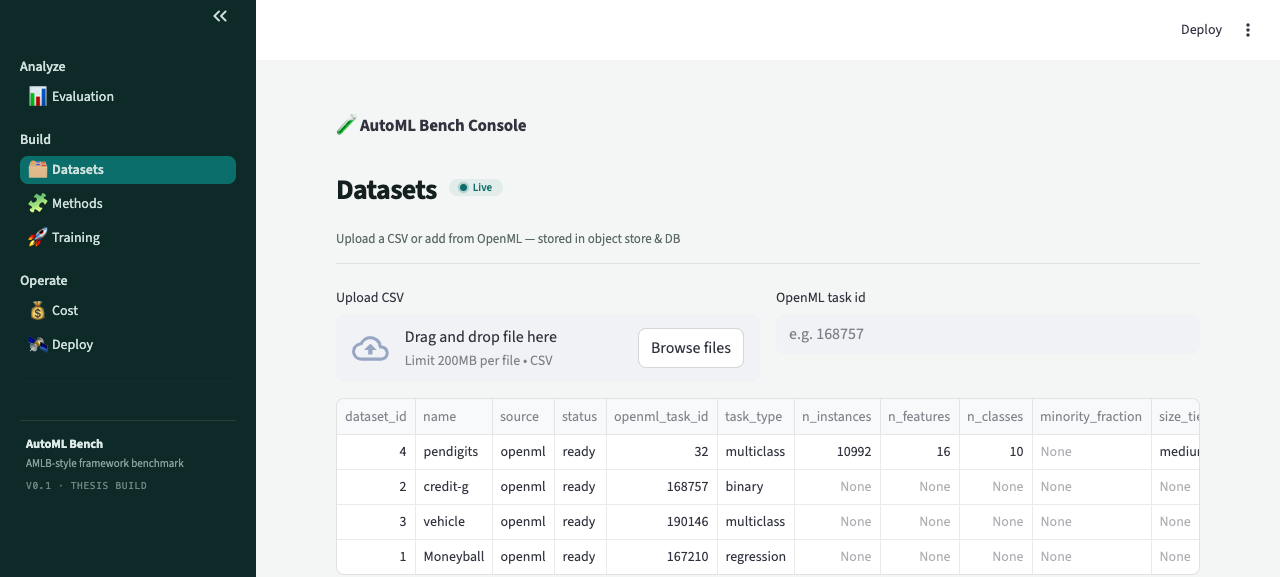
\includegraphics[width=0.88\linewidth]{image/console-datasets.png}
    \caption{Khu vực quản lý dữ liệu: nạp bộ dữ liệu từ tệp CSV, tác vụ OpenML
    hoặc liên kết Kaggle công khai.}
    \label{fig:console-datasets}
\end{figure}

Khu vực quản lý thư viện (Hình~\ref{fig:console-methods}) hiển thị danh mục các
thư viện AutoML kèm trạng thái tích hợp và mức độ tương thích với cấu hình máy
hiện tại. Trạng thái được báo cáo trung thực theo kết quả kiểm tra thực tế thay vì
giả định, nhờ đó người dùng biết trước thư viện nào có thể chạy được trên máy của
mình trước khi khởi động một lượt đánh giá kéo dài nhiều giờ.

\begin{figure}[H]
    \centering
    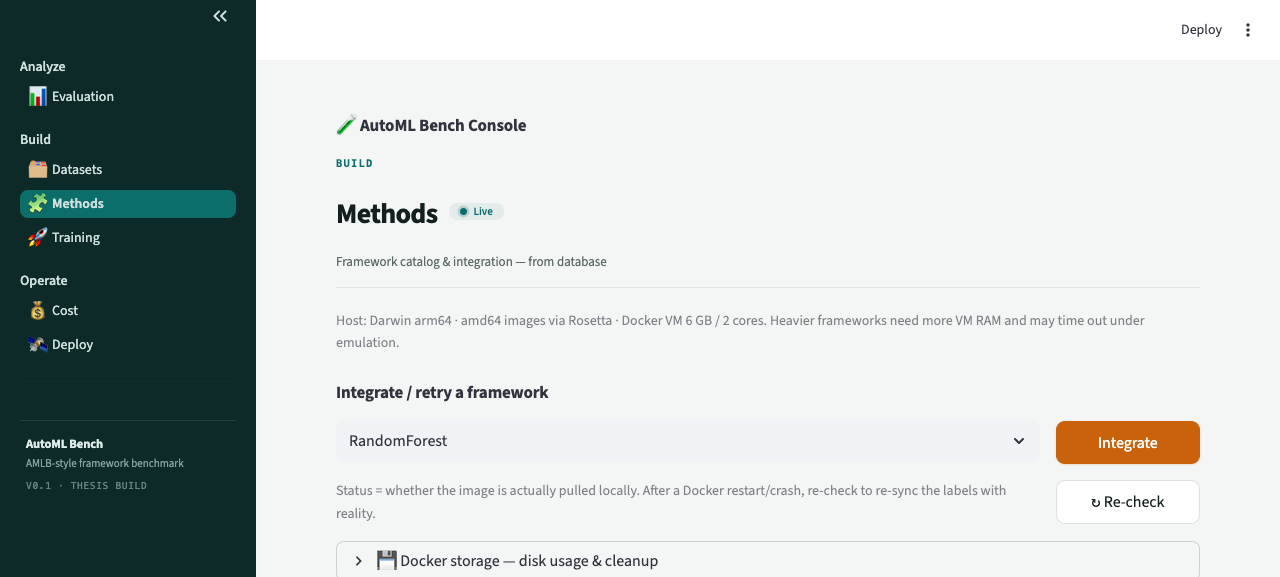
\includegraphics[width=0.88\linewidth]{image/console-methods.png}
    \caption{Khu vực quản lý thư viện: danh mục các thư viện AutoML kèm trạng thái
    tích hợp và phù hiệu tương thích theo cấu hình máy.}
    \label{fig:console-methods}
\end{figure}

Khu vực khởi chạy (Hình~\ref{fig:console-training}) cho phép chọn tổ hợp thư viện,
bộ dữ liệu và ngân sách thời gian, sau đó khởi động lượt đánh giá và theo dõi
trạng thái từng công việc theo thời gian thực. Cuối cùng, khu vực tổng hợp kết quả
(Hình~\ref{fig:console-eval}) trình bày bảng xếp hạng, biểu đồ đánh đổi giữa chất
lượng và thời gian, cùng khung nhìn phân tích theo đặc trưng bộ dữ liệu.

\begin{figure}[H]
    \centering
    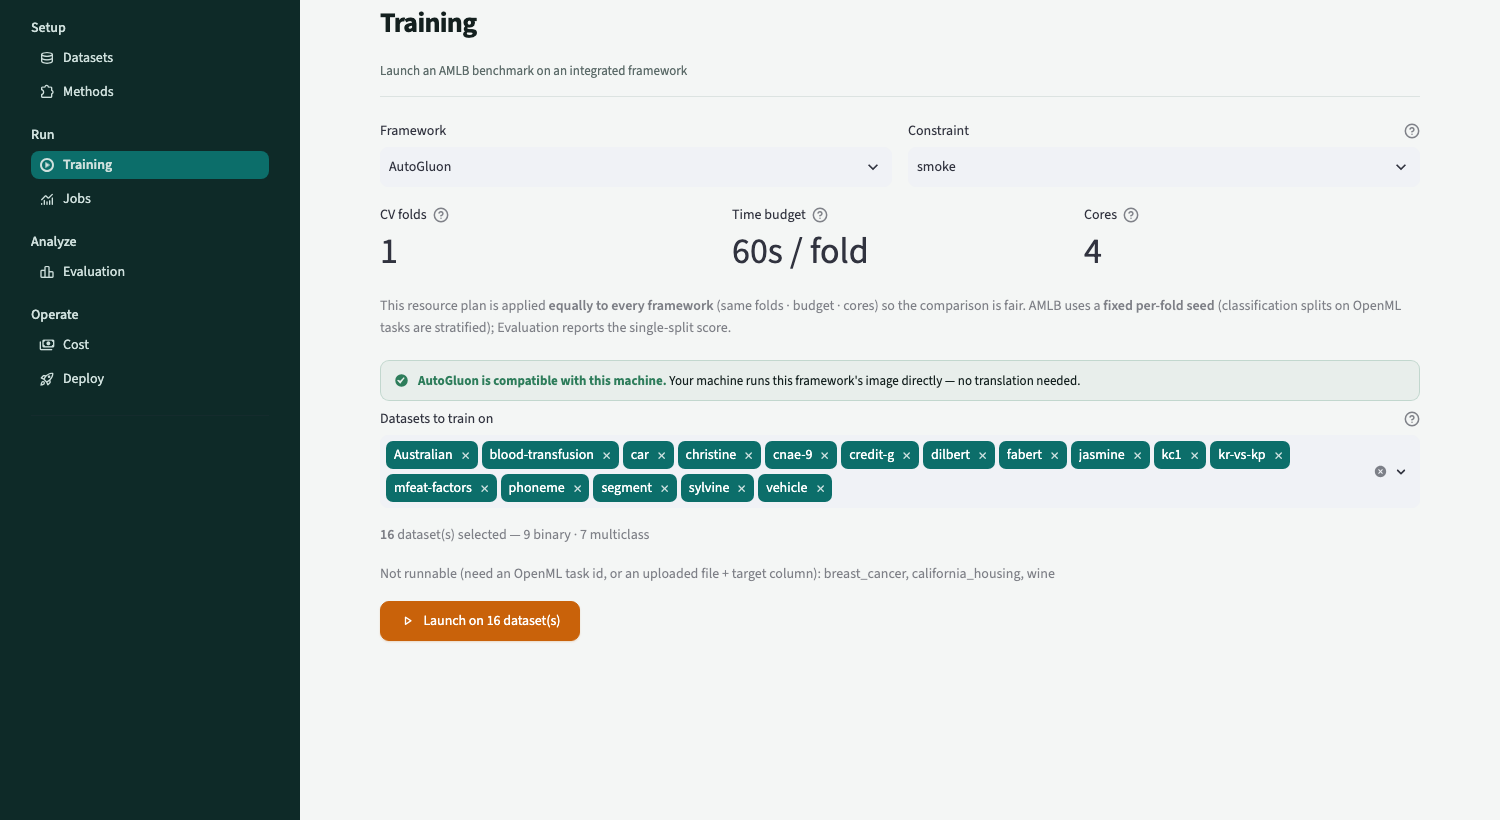
\includegraphics[width=0.88\linewidth]{image/console-training.png}
    \caption{Khu vực khởi chạy: lựa chọn thư viện, bộ dữ liệu và ngân sách thời
    gian, đồng thời theo dõi trạng thái các công việc đang thực thi.}
    \label{fig:console-training}
\end{figure}

\begin{figure}[H]
    \centering
    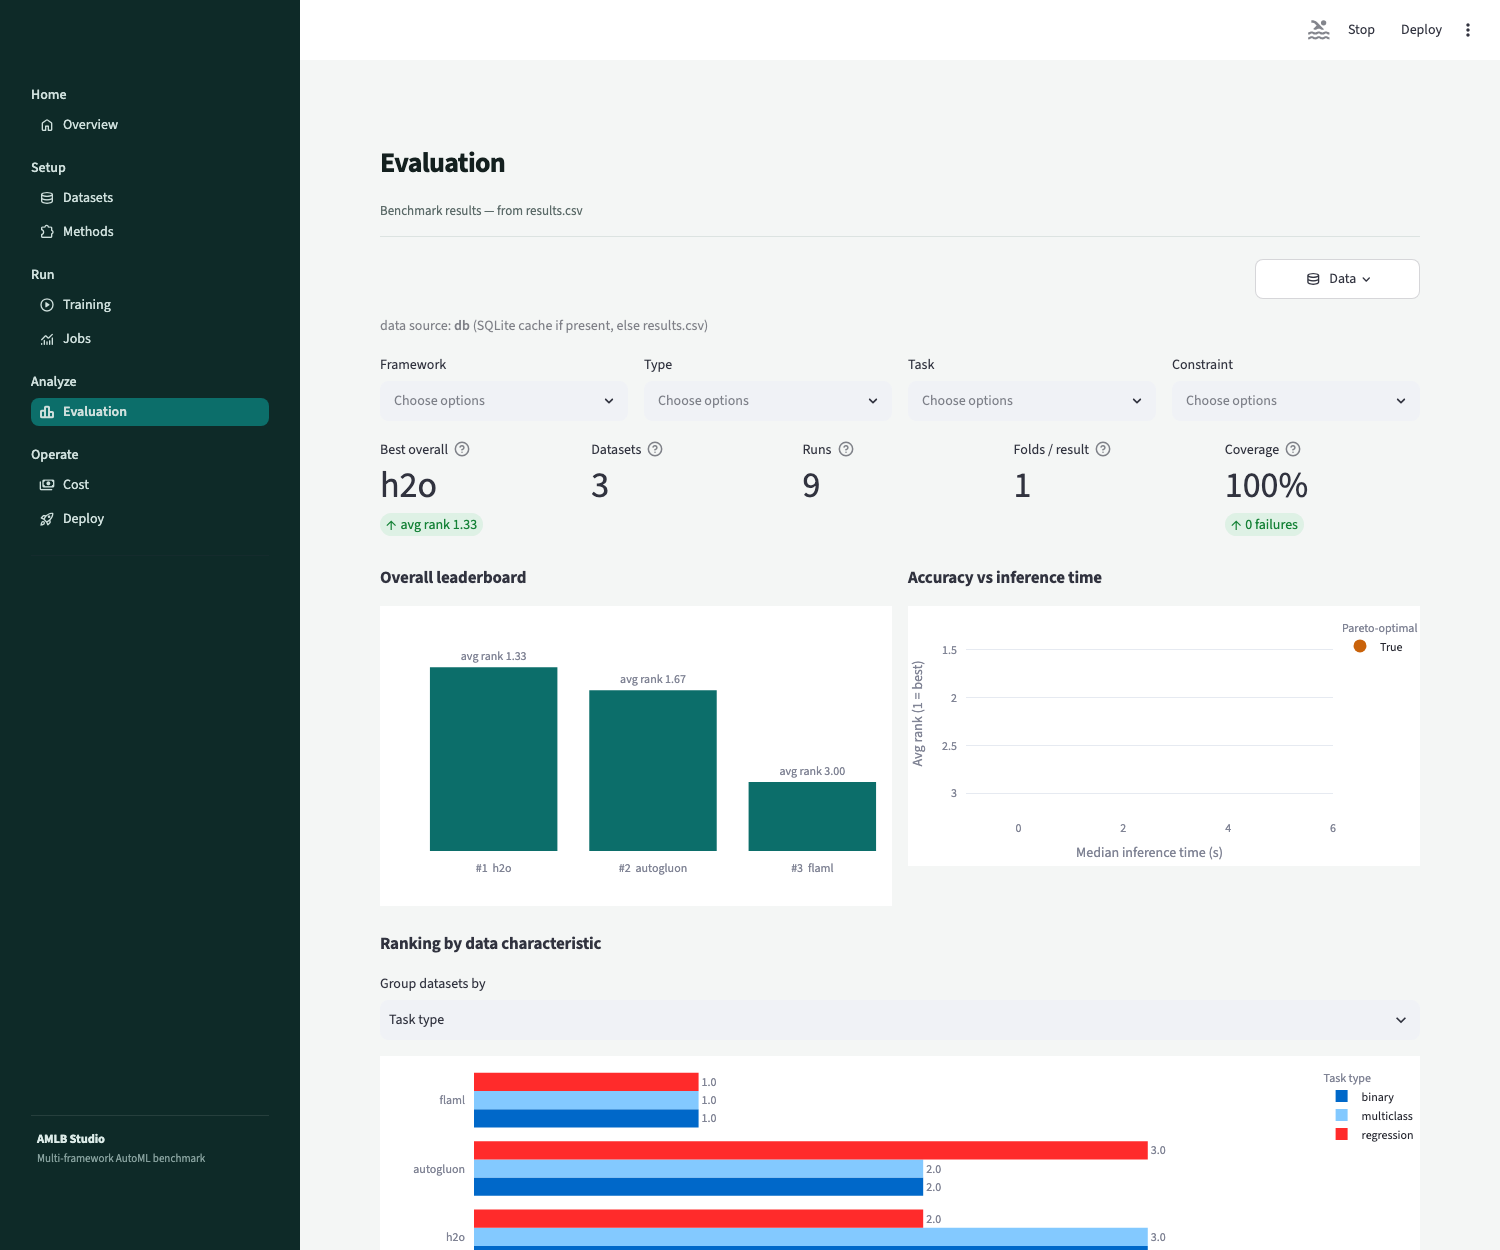
\includegraphics[width=0.88\linewidth]{image/eval-dashboard.png}
    \caption{Khu vực tổng hợp kết quả: bảng xếp hạng, biểu đồ đánh đổi chất lượng
    -- thời gian và khung nhìn theo đặc trưng bộ dữ liệu.}
    \label{fig:console-eval}
\end{figure}

Cần lưu ý rằng giao diện này đóng vai trò công cụ hỗ trợ khảo sát và trình diễn;
toàn bộ kết quả trình bày ở Chương~\ref{ch:thucnghiem} được tạo ra bằng bộ công cụ
dòng lệnh mô tả ở Mục~\ref{sec:kientruc}, vốn phù hợp hơn với việc chạy phân tán
trên nhiều máy trong thời gian dài.

\section{Thảo luận về các lựa chọn thiết kế}
\label{sec:thaoluan-pp}
Việc tách bạch giữa \emph{giao thức} và \emph{hiện thực} là lựa chọn thiết kế
trung tâm. Giao thức quy định các bất biến cần được bảo toàn để phép so sánh có
giá trị, còn hiện thực có thể thay đổi mà không ảnh hưởng tới tính đúng đắn của
kết luận.

Lựa chọn cô lập môi trường bằng môi trường ảo riêng cho từng thư viện, thay vì
đóng gói bằng container, xuất phát từ ràng buộc thực tế: khối lượng tính toán được
chia trên các máy cá nhân của thành viên nhóm cũng như trên nền tảng đám mây miễn
phí, nơi việc chạy container không phải lúc nào cũng khả dụng. Đánh đổi của lựa
chọn này là mức độ cô lập thấp hơn container ở tầng thư viện hệ thống; tuy nhiên,
vì mọi thư viện đều được đánh giá trên cùng một máy với cùng cấu hình phần cứng
trong mỗi lượt chạy, điều kiện công bằng theo Định nghĩa~\ref{def:congbang} vẫn
được bảo toàn.

Cơ chế khôi phục sau gián đoạn cũng là một yêu cầu bắt buộc chứ không phải tiện
ích phụ. Với thời gian chạy lên tới hàng chục giờ máy, xác suất gặp gián đoạn là
đáng kể; nếu không có khả năng tiếp tục từ điểm dừng, mỗi lần gián đoạn sẽ buộc
phải chạy lại từ đầu và làm cho thực nghiệm quy mô này trở nên bất khả thi.

Cuối cùng, quyết định giữ bước tiền xử lý ở mức tối thiểu phản ánh đúng mục tiêu
đánh giá. Nếu nhóm thực hiện mã hoá biến hạng mục hay điền giá trị khuyết một cách
công phu trước khi đưa vào các thư viện, phần năng lực xử lý dữ liệu thô --- vốn
là một thành phần quan trọng của AutoML --- sẽ bị che khuất, và kết quả so sánh
chỉ còn phản ánh năng lực tìm kiếm siêu tham số.

\section{Các yếu tố đe doạ tính hợp lệ và biện pháp kiểm soát}
\label{sec:hopleimuc}
Một thiết kế thực nghiệm chặt chẽ đòi hỏi nhận diện trước những yếu tố có thể làm
sai lệch kết luận. Bảng~\ref{tab:threats} liệt kê các yếu tố đã được nhóm nhận
diện cùng biện pháp kiểm soát tương ứng.

\begin{table}[H]
  \centering
  \small
  \caption{Các yếu tố đe doạ tính hợp lệ của kết luận và biện pháp kiểm soát.}
  \label{tab:threats}
  \renewcommand{\arraystretch}{1.25}
  \begin{tabularx}{\linewidth}{@{}>{\raggedright\arraybackslash}p{4.2cm} X@{}}
    \toprule
    \textbf{Yếu tố đe doạ} & \textbf{Biện pháp kiểm soát} \\
    \midrule
    Phương sai do phép chia dữ liệu &
    Phân hoạch fold sinh một lần từ hạt giống cố định, dùng chung cho mọi thư
    viện; phân tầng theo nhãn với bài toán phân loại. \\
    Xung đột phiên bản thư viện phụ thuộc &
    Mỗi thư viện được cài đặt và thực thi trong một môi trường ảo Python riêng
    biệt. \\
    Ngân sách tài nguyên không đồng nhất &
    Cùng một giá trị ngân sách được truyền vào tham số của mọi thư viện, kèm
    ngưỡng cứng do tiến trình cha áp đặt. \\
    Thiên lệch sống sót do bỏ qua thất bại &
    Mọi lần chạy đều sinh bản ghi; các lần thất bại được giữ lại kèm phân loại
    nguyên nhân và được phân tích riêng. \\
    Khác biệt phần cứng giữa các máy &
    Toàn bộ các thư viện trên cùng một bộ dữ liệu được chạy trên cùng một máy;
    việc phân tán được thực hiện theo chiều bộ dữ liệu chứ không cắt ngang một
    phép so sánh. \\
    Kết luận dựa trên chênh lệch không đáng kể &
    Báo cáo kèm độ lệch chuẩn giữa các fold; không tuyên bố hơn kém khi chênh
    lệch nằm dưới ngưỡng độ lệch chuẩn quan sát được. \\
    Thang đo khác nhau giữa các bộ dữ liệu &
    Xếp hạng dựa trên mô hình Bradley--Terry, vốn chỉ sử dụng quan hệ thứ tự nên
    bất biến với phép biến đổi đơn điệu của thang đo. \\
    \bottomrule
  \end{tabularx}
\end{table}

Yếu tố thứ năm trong bảng đáng được nhấn mạnh. Khi phân tán khối lượng tính toán
trên nhiều máy có cấu hình khác nhau, nếu chia việc theo chiều \emph{thư viện} thì
hai thư viện được so sánh có thể chạy trên hai máy khác nhau, và chênh lệch thời
gian quan sát được sẽ phản ánh sự khác biệt phần cứng chứ không phải thuật toán.
Vì vậy việc phân tán được thực hiện sao cho mọi thư viện trên cùng một bộ dữ liệu
luôn được đánh giá trên cùng một máy, giữ nguyên tính hợp lệ của phép so sánh
trong phạm vi từng bộ dữ liệu.
